\documentclass{standalone}
\usepackage{tikz}
\usetikzlibrary{patterns, positioning}


\begin{document}
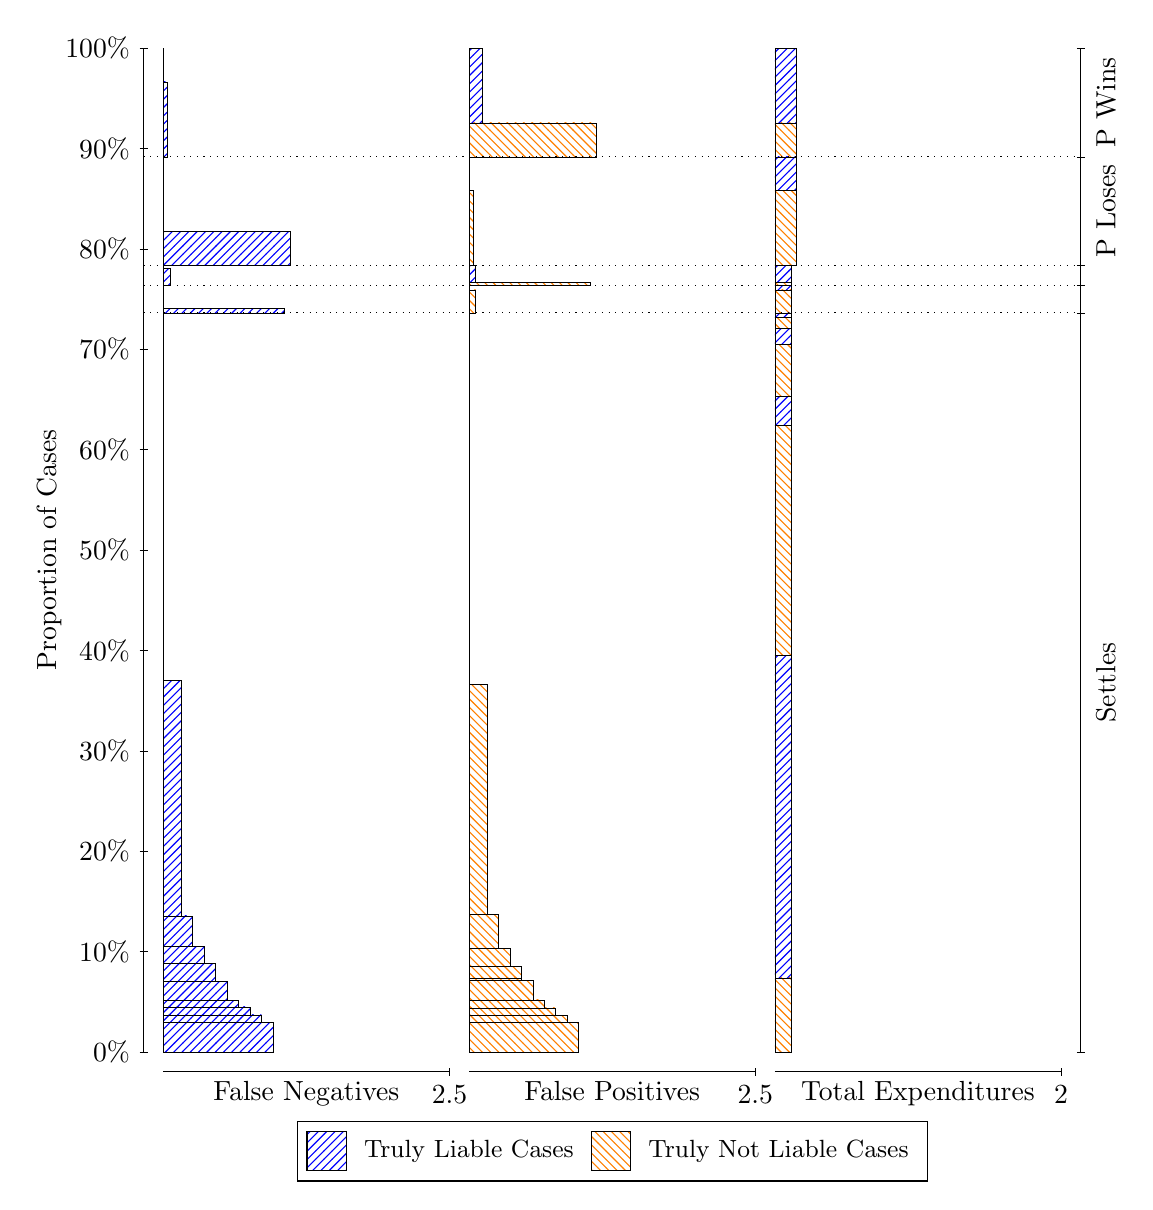
\begin{tikzpicture}
\draw[black, very thin] (1.5,1.75) -- (1.5,14.5);
\node[rotate=90, text=black, anchor=center] at (0.3, 8.125) {Proportion of Cases};
\draw[black, very thin] (1.45,1.75) -- (1.55,1.75);
\node[text=black, anchor=east] at (1.45, 1.75) {0\%};
\draw[black, very thin] (1.45,3.025) -- (1.55,3.025);
\node[text=black, anchor=east] at (1.45, 3.025) {10\%};
\draw[black, very thin] (1.45,4.3) -- (1.55,4.3);
\node[text=black, anchor=east] at (1.45, 4.3) {20\%};
\draw[black, very thin] (1.45,5.575) -- (1.55,5.575);
\node[text=black, anchor=east] at (1.45, 5.575) {30\%};
\draw[black, very thin] (1.45,6.85) -- (1.55,6.85);
\node[text=black, anchor=east] at (1.45, 6.85) {40\%};
\draw[black, very thin] (1.45,8.125) -- (1.55,8.125);
\node[text=black, anchor=east] at (1.45, 8.125) {50\%};
\draw[black, very thin] (1.45,9.4) -- (1.55,9.4);
\node[text=black, anchor=east] at (1.45, 9.4) {60\%};
\draw[black, very thin] (1.45,10.675) -- (1.55,10.675);
\node[text=black, anchor=east] at (1.45, 10.675) {70\%};
\draw[black, very thin] (1.45,11.95) -- (1.55,11.95);
\node[text=black, anchor=east] at (1.45, 11.95) {80\%};
\draw[black, very thin] (1.45,13.225) -- (1.55,13.225);
\node[text=black, anchor=east] at (1.45, 13.225) {90\%};
\draw[black, very thin] (1.45,14.5) -- (1.55,14.5);
\node[text=black, anchor=east] at (1.45, 14.5) {100\%};

\draw[black, very thin] (13.4,1.75) -- (13.4,14.5);
\draw[black, very thin] (13.35,1.75) -- (13.45,1.75);
\node[anchor=west] at (13.35, 1.75) {};
\draw[black, very thin] (13.35,11.137) -- (13.45,11.137);
\node[anchor=west] at (13.35, 11.137) {};
\draw[black, very thin] (13.35,11.484) -- (13.45,11.484);
\node[anchor=west] at (13.35, 11.484) {};
\draw[black, very thin] (13.35,11.74) -- (13.45,11.74);
\node[anchor=west] at (13.35, 11.74) {};
\draw[black, very thin] (13.35,13.118) -- (13.45,13.118);
\node[anchor=west] at (13.35, 13.118) {};
\draw[black, very thin] (13.35,14.5) -- (13.45,14.5);
\node[anchor=west] at (13.35, 14.5) {};

\draw[black, very thin, pattern color=blue, pattern=north east lines] (1.75,1.75) rectangle (3.1398,2.1209);
\draw[black, very thin, pattern color=blue, pattern=north east lines] (1.75,2.1209) rectangle (2.9944,2.2203);
\draw[black, very thin, pattern color=blue, pattern=north east lines] (1.75,2.2203) rectangle (2.8491,2.3213);
\draw[black, very thin, pattern color=blue, pattern=north east lines] (1.75,2.3213) rectangle (2.7037,2.4059);
\draw[black, very thin, pattern color=blue, pattern=north east lines] (1.75,2.4059) rectangle (2.5584,2.6487);
\draw[black, very thin, pattern color=blue, pattern=north east lines] (1.75,2.6487) rectangle (2.4131,2.8758);
\draw[black, very thin, pattern color=blue, pattern=north east lines] (1.75,2.8758) rectangle (2.2678,3.0918);
\draw[black, very thin, pattern color=blue, pattern=north east lines] (1.75,3.0918) rectangle (2.1224,3.4785);
\draw[black, very thin, pattern color=blue, pattern=north east lines] (1.75,3.4785) rectangle (1.9771,6.4716);
\draw[black, very thin, pattern color=orange, pattern=north west lines] (1.75,6.4716) rectangle (1.75,11.137);
\draw[black, very thin, pattern color=blue, pattern=north east lines] (1.75,11.137) rectangle (3.2851,11.194);
\draw[black, very thin, pattern color=orange, pattern=north west lines] (1.75,11.194) rectangle (1.75,11.484);
\draw[black, very thin, pattern color=blue, pattern=north east lines] (1.75,11.484) rectangle (1.8318,11.698);
\draw[black, very thin, pattern color=orange, pattern=north west lines] (1.75,11.698) rectangle (1.75,11.74);
\draw[black, very thin, pattern color=blue, pattern=north east lines] (1.75,11.74) rectangle (3.3668,12.171);
\draw[black, very thin, pattern color=orange, pattern=north west lines] (1.75,12.171) rectangle (1.75,13.118);
\draw[black, very thin, pattern color=blue, pattern=north east lines] (1.75,13.118) rectangle (1.8045,14.07);
\draw[black, very thin, pattern color=orange, pattern=north west lines] (1.75,14.07) rectangle (1.75,14.5);
\draw[black, very thin, pattern color=orange, pattern=north west lines] (5.6333,1.75) rectangle (7.0231,2.1296);
\draw[black, very thin, pattern color=orange, pattern=north west lines] (5.6333,2.1296) rectangle (6.8777,2.2193);
\draw[black, very thin, pattern color=orange, pattern=north west lines] (5.6333,2.2193) rectangle (6.7324,2.3098);
\draw[black, very thin, pattern color=orange, pattern=north west lines] (5.6333,2.3098) rectangle (6.5871,2.4103);
\draw[black, very thin, pattern color=orange, pattern=north west lines] (5.6333,2.4103) rectangle (6.4417,2.6556);
\draw[black, very thin, pattern color=orange, pattern=north west lines] (5.6333,2.6556) rectangle (6.2964,2.6896);
\draw[black, very thin, pattern color=orange, pattern=north west lines] (5.6333,2.6896) rectangle (6.2964,2.8348);
\draw[black, very thin, pattern color=orange, pattern=north west lines] (5.6333,2.8348) rectangle (6.1511,3.0637);
\draw[black, very thin, pattern color=orange, pattern=north west lines] (5.6333,3.0637) rectangle (6.0057,3.4959);
\draw[black, very thin, pattern color=orange, pattern=north west lines] (5.6333,3.4959) rectangle (5.8604,6.4155);
\draw[black, very thin, pattern color=blue, pattern=north east lines] (5.6333,6.4155) rectangle (5.6333,11.137);
\draw[black, very thin, pattern color=orange, pattern=north west lines] (5.6333,11.137) rectangle (5.7151,11.427);
\draw[black, very thin, pattern color=blue, pattern=north east lines] (5.6333,11.427) rectangle (5.6333,11.484);
\draw[black, very thin, pattern color=orange, pattern=north west lines] (5.6333,11.484) rectangle (7.1684,11.526);
\draw[black, very thin, pattern color=blue, pattern=north east lines] (5.6333,11.526) rectangle (5.7151,11.74);
\draw[black, very thin, pattern color=orange, pattern=north west lines] (5.6333,11.74) rectangle (5.6878,12.688);
\draw[black, very thin, pattern color=blue, pattern=north east lines] (5.6333,12.688) rectangle (5.6333,13.118);
\draw[black, very thin, pattern color=orange, pattern=north west lines] (5.6333,13.118) rectangle (7.2502,13.548);
\draw[black, very thin, pattern color=blue, pattern=north east lines] (5.6333,13.548) rectangle (5.7968,14.5);
\draw[black, very thin, pattern color=orange, pattern=north west lines] (9.5167,1.75) rectangle (9.721,2.6896);
\draw[black, very thin, pattern color=blue, pattern=north east lines] (9.5167,2.6896) rectangle (9.721,6.7863);
\draw[black, very thin, pattern color=orange, pattern=north west lines] (9.5167,6.7863) rectangle (9.721,9.7058);
\draw[black, very thin, pattern color=blue, pattern=north east lines] (9.5167,9.7058) rectangle (9.721,10.077);
\draw[black, very thin, pattern color=orange, pattern=north west lines] (9.5167,10.077) rectangle (9.721,10.738);
\draw[black, very thin, pattern color=blue, pattern=north east lines] (9.5167,10.738) rectangle (9.721,10.938);
\draw[black, very thin, pattern color=orange, pattern=north west lines] (9.5167,10.938) rectangle (9.721,11.083);
\draw[black, very thin, pattern color=blue, pattern=north east lines] (9.5167,11.083) rectangle (9.721,11.137);
\draw[black, very thin, pattern color=orange, pattern=north west lines] (9.5167,11.137) rectangle (9.721,11.427);
\draw[black, very thin, pattern color=blue, pattern=north east lines] (9.5167,11.427) rectangle (9.721,11.484);
\draw[black, very thin, pattern color=orange, pattern=north west lines] (9.5167,11.484) rectangle (9.721,11.526);
\draw[black, very thin, pattern color=blue, pattern=north east lines] (9.5167,11.526) rectangle (9.721,11.74);
\draw[black, very thin, pattern color=orange, pattern=north west lines] (9.5167,11.74) rectangle (9.7892,12.688);
\draw[black, very thin, pattern color=blue, pattern=north east lines] (9.5167,12.688) rectangle (9.7892,13.118);
\draw[black, very thin, pattern color=orange, pattern=north west lines] (9.5167,13.118) rectangle (9.7892,13.548);
\draw[black, very thin, pattern color=blue, pattern=north east lines] (9.5167,13.548) rectangle (9.7892,14.5);
\draw[black, dotted] (1.5,11.137) -- (13.4,11.137);
\draw[black, dotted] (1.5,11.484) -- (13.4,11.484);
\draw[black, dotted] (1.5,11.74) -- (13.4,11.74);
\draw[black, dotted] (1.5,13.118) -- (13.4,13.118);
\draw[black, very thin] (1.75,1.5) -- (5.3833,1.5);
\node[text=black, anchor=north] at (3.5667, 1.5) {False Negatives};
\draw[black, very thin] (5.3833,1.45) -- (5.3833,1.55);
\node[text=black, anchor=north] at (5.3833, 1.45) {2.5};

\draw[black, very thin] (5.6333,1.5) -- (9.2667,1.5);
\node[text=black, anchor=north] at (7.45, 1.5) {False Positives};
\draw[black, very thin] (9.2667,1.45) -- (9.2667,1.55);
\node[text=black, anchor=north] at (9.2667, 1.45) {2.5};

\draw[black, very thin] (9.5167,1.5) -- (13.15,1.5);
\node[text=black, anchor=north] at (11.333, 1.5) {Total Expenditures};
\draw[black, very thin] (13.15,1.45) -- (13.15,1.55);
\node[text=black, anchor=north] at (13.15, 1.45) {2};

\node[text=black, centered, rotate=90] at (13.72, 6.4435) {Settles};


\node[text=black, centered, rotate=90] at (13.72, 12.429) {P Loses};
\node[text=black, centered, rotate=90] at (13.72, 13.809) {P Wins};

\draw (7.449999999999999,1.5) node[draw=none] (baseCoordinate) {};
\begin{scope}[align=center]
        \matrix[scale=0.5, draw=black, below=0.5cm of baseCoordinate, nodes={draw}, column sep=0.1cm]{
            \node[rectangle, draw, minimum width=0.5cm, minimum height=0.5cm, pattern color=blue, pattern=north east lines] {}; &
            \node[draw=none, font=\small, text=black] (B) {Truly Liable Cases}; &
            \node[rectangle, draw, minimum width=0.5cm, minimum height=0.5cm, pattern color=orange, pattern=north west lines] {}; &
            \node[draw=none, font=\small, text=black] (B) {Truly Not Liable Cases}; \\
            };
\end{scope}

\end{tikzpicture}
\end{document}